\begin{frame}
    \frametitle{Planning Transfe}
    \begin{block}{}
        Finally achieved a stable low earth orbit. We need to plan our tranfer to our target body
    \end{block}
\end{frame}
\begin{frame}
    \begin{center}
        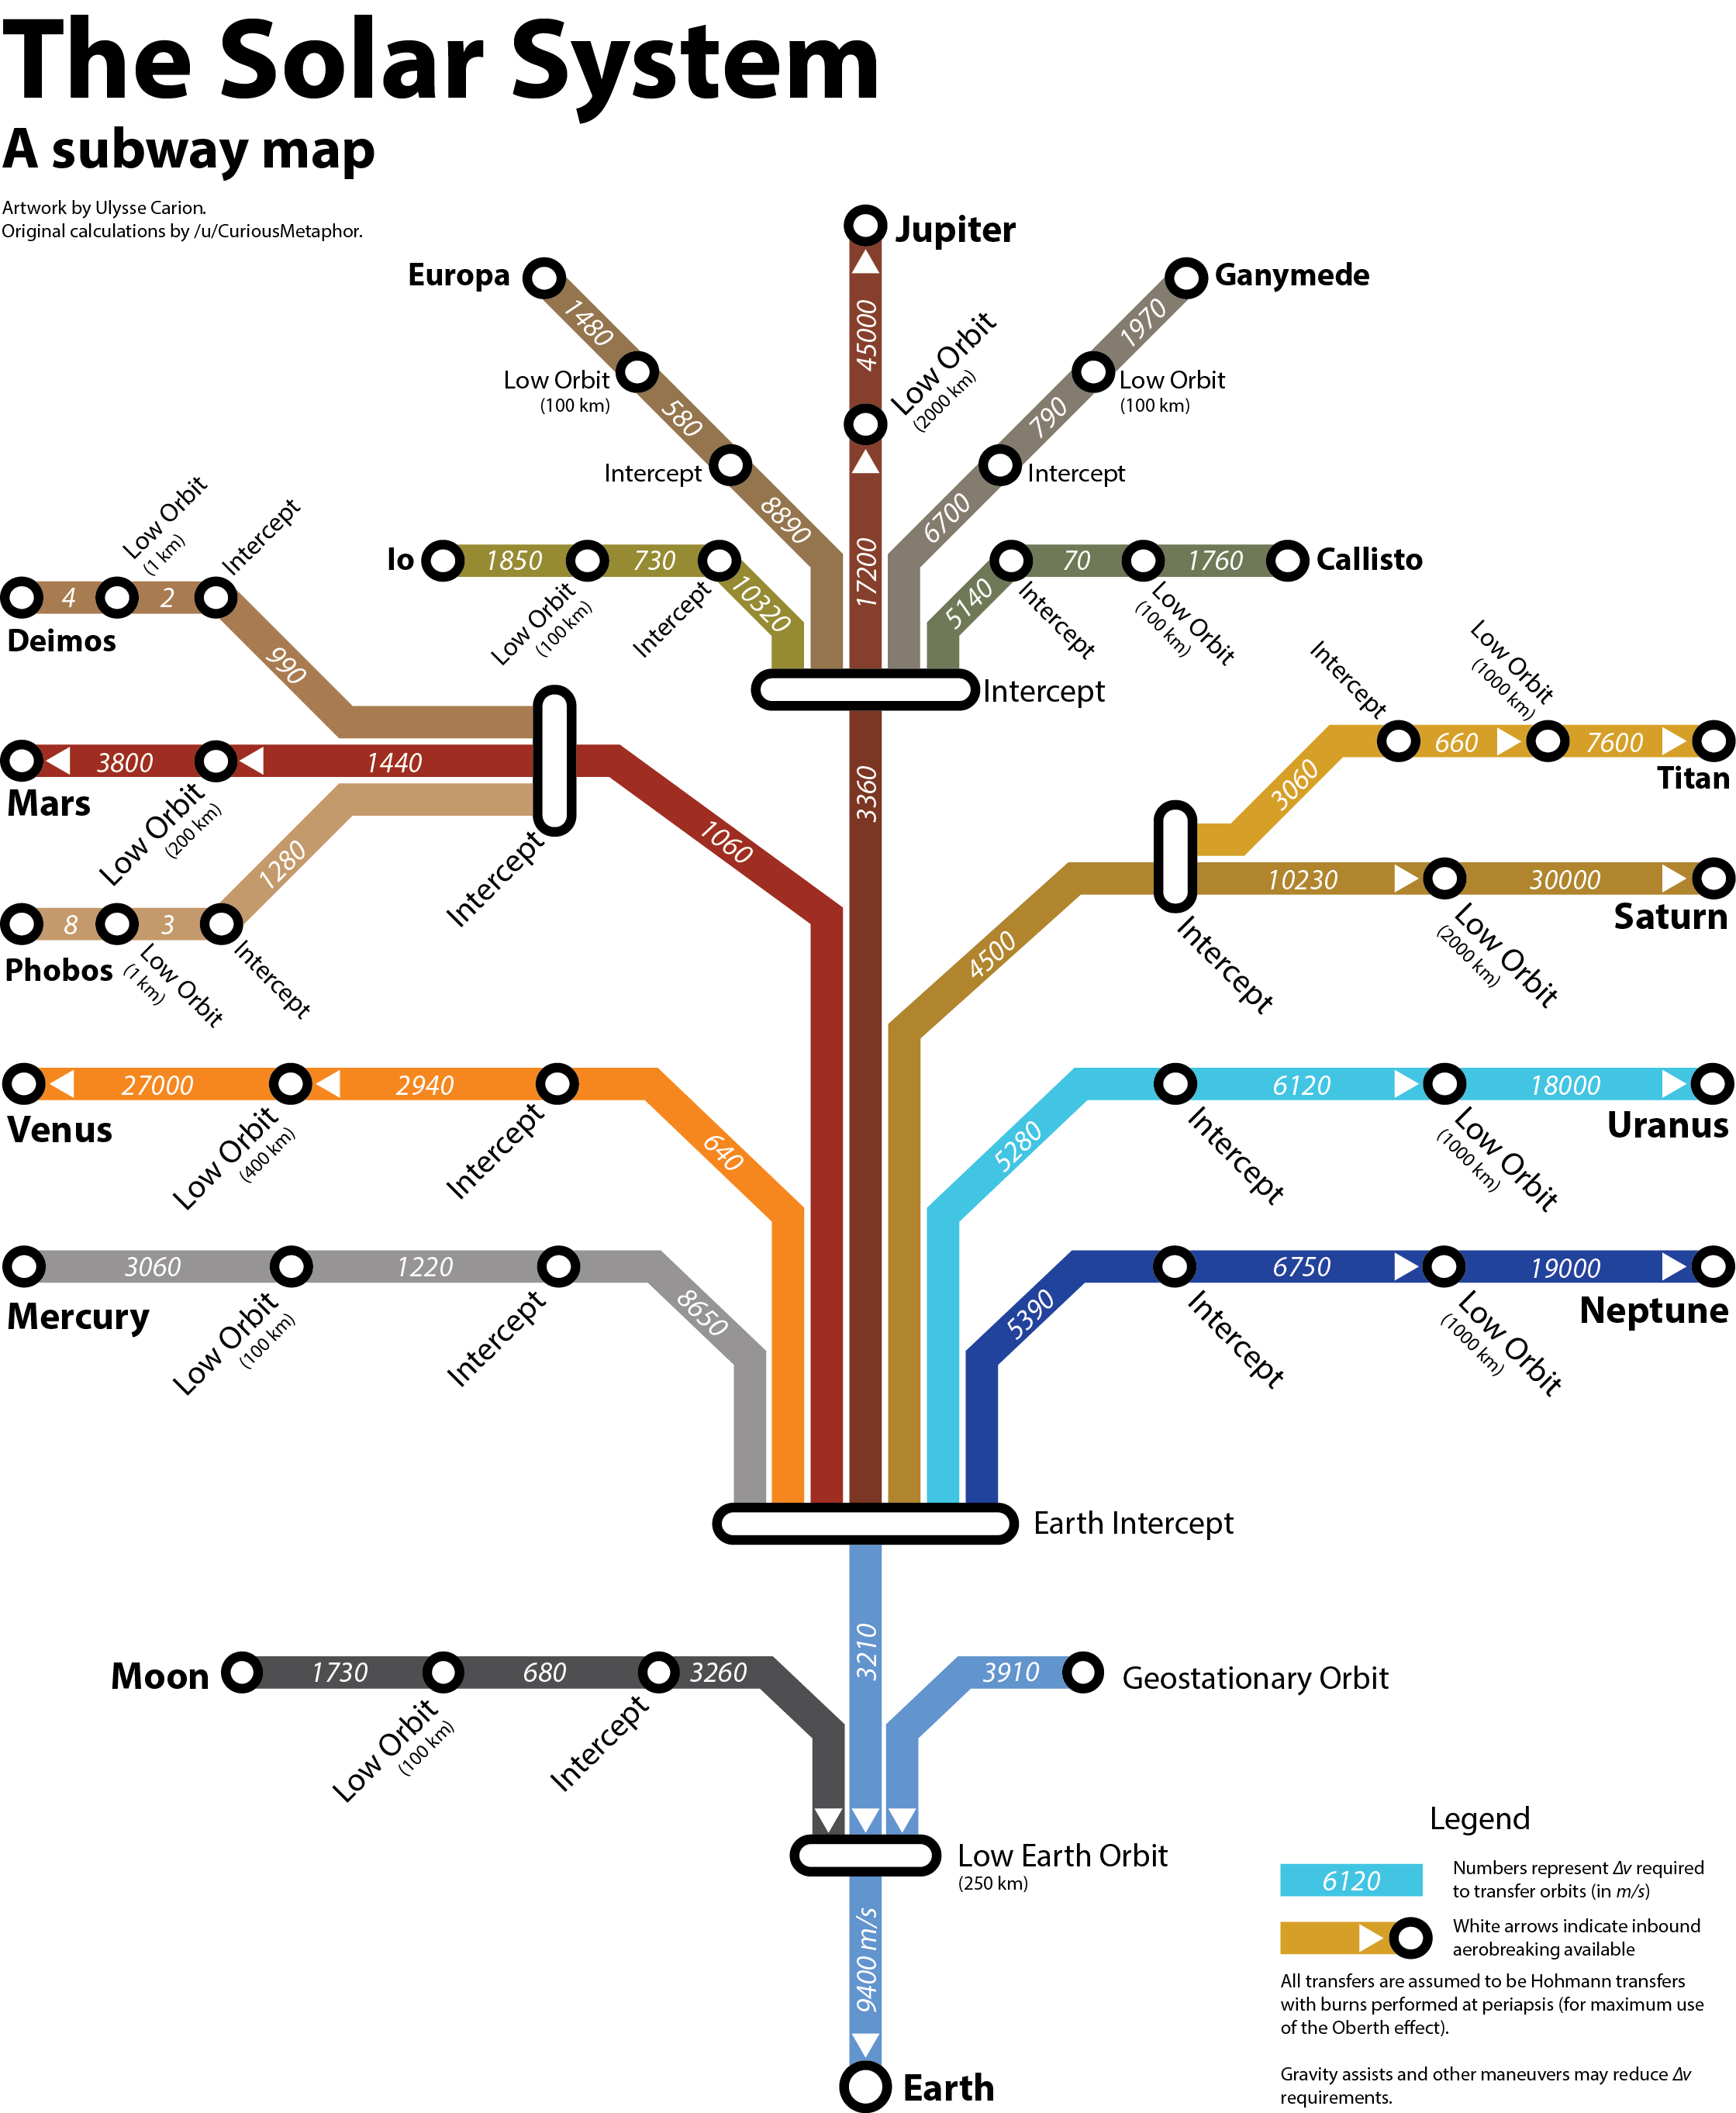
\includegraphics[height=\textheight]{images/deltavmap.png}
    \end{center}
\end{frame}
\begin{frame}
    \frametitle{Hohmann transfer}
    \begin{block}{}
        Now that we now our target and know the delta-v required to get there we need to plan the encounter
    \end{block}
    \begin{block}{}
        \begin{center}
            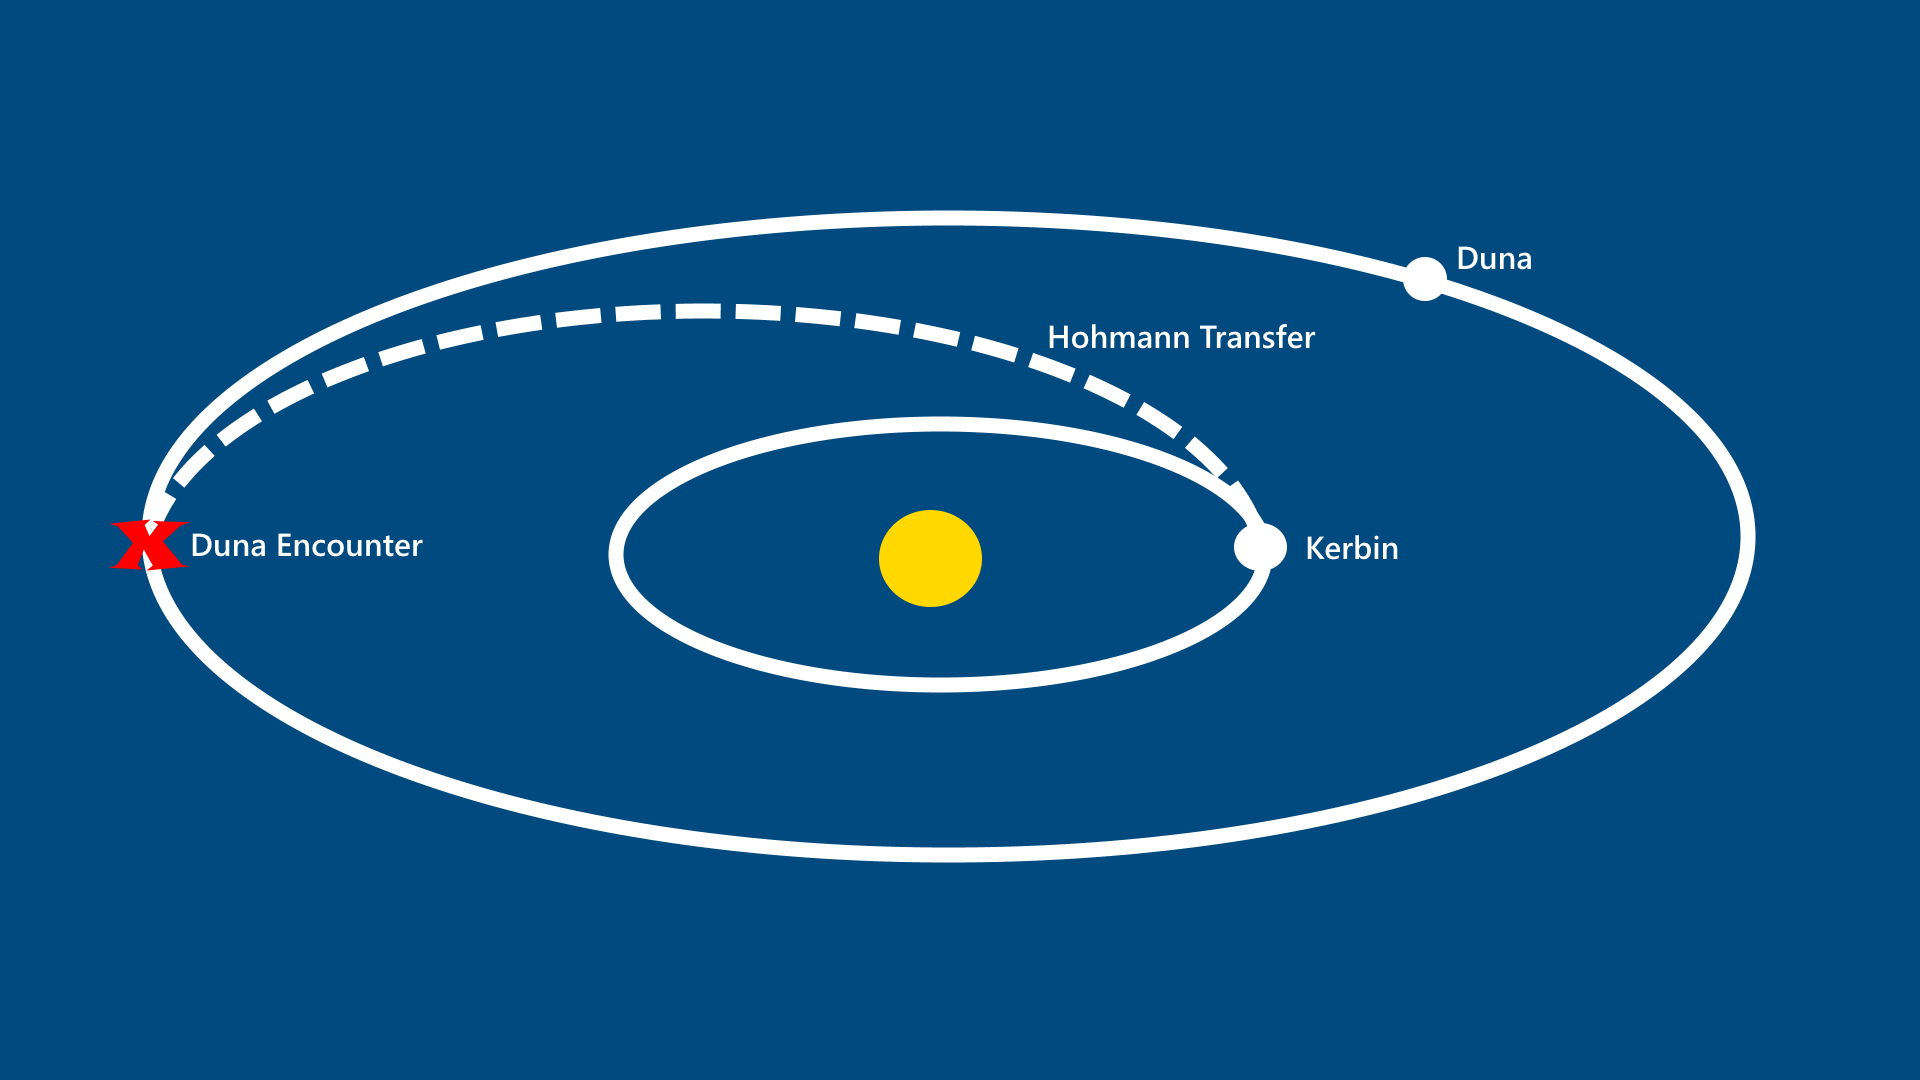
\includegraphics[scale=0.2]{images/hohmann_transfer}
        \end{center}
    \end{block}
\end{frame}
\begin{frame}
    \frametitle{Hohmann transfer window}
    \begin{block}{}
        To be able to transfer with the least amount of delta-v as possible we need to launch when the target body is
        at an exact position relative to us. If we are on a strict delta-v budget we need to wait for a good window
    \end{block}
    \begin{block}{}
        \begin{center}
            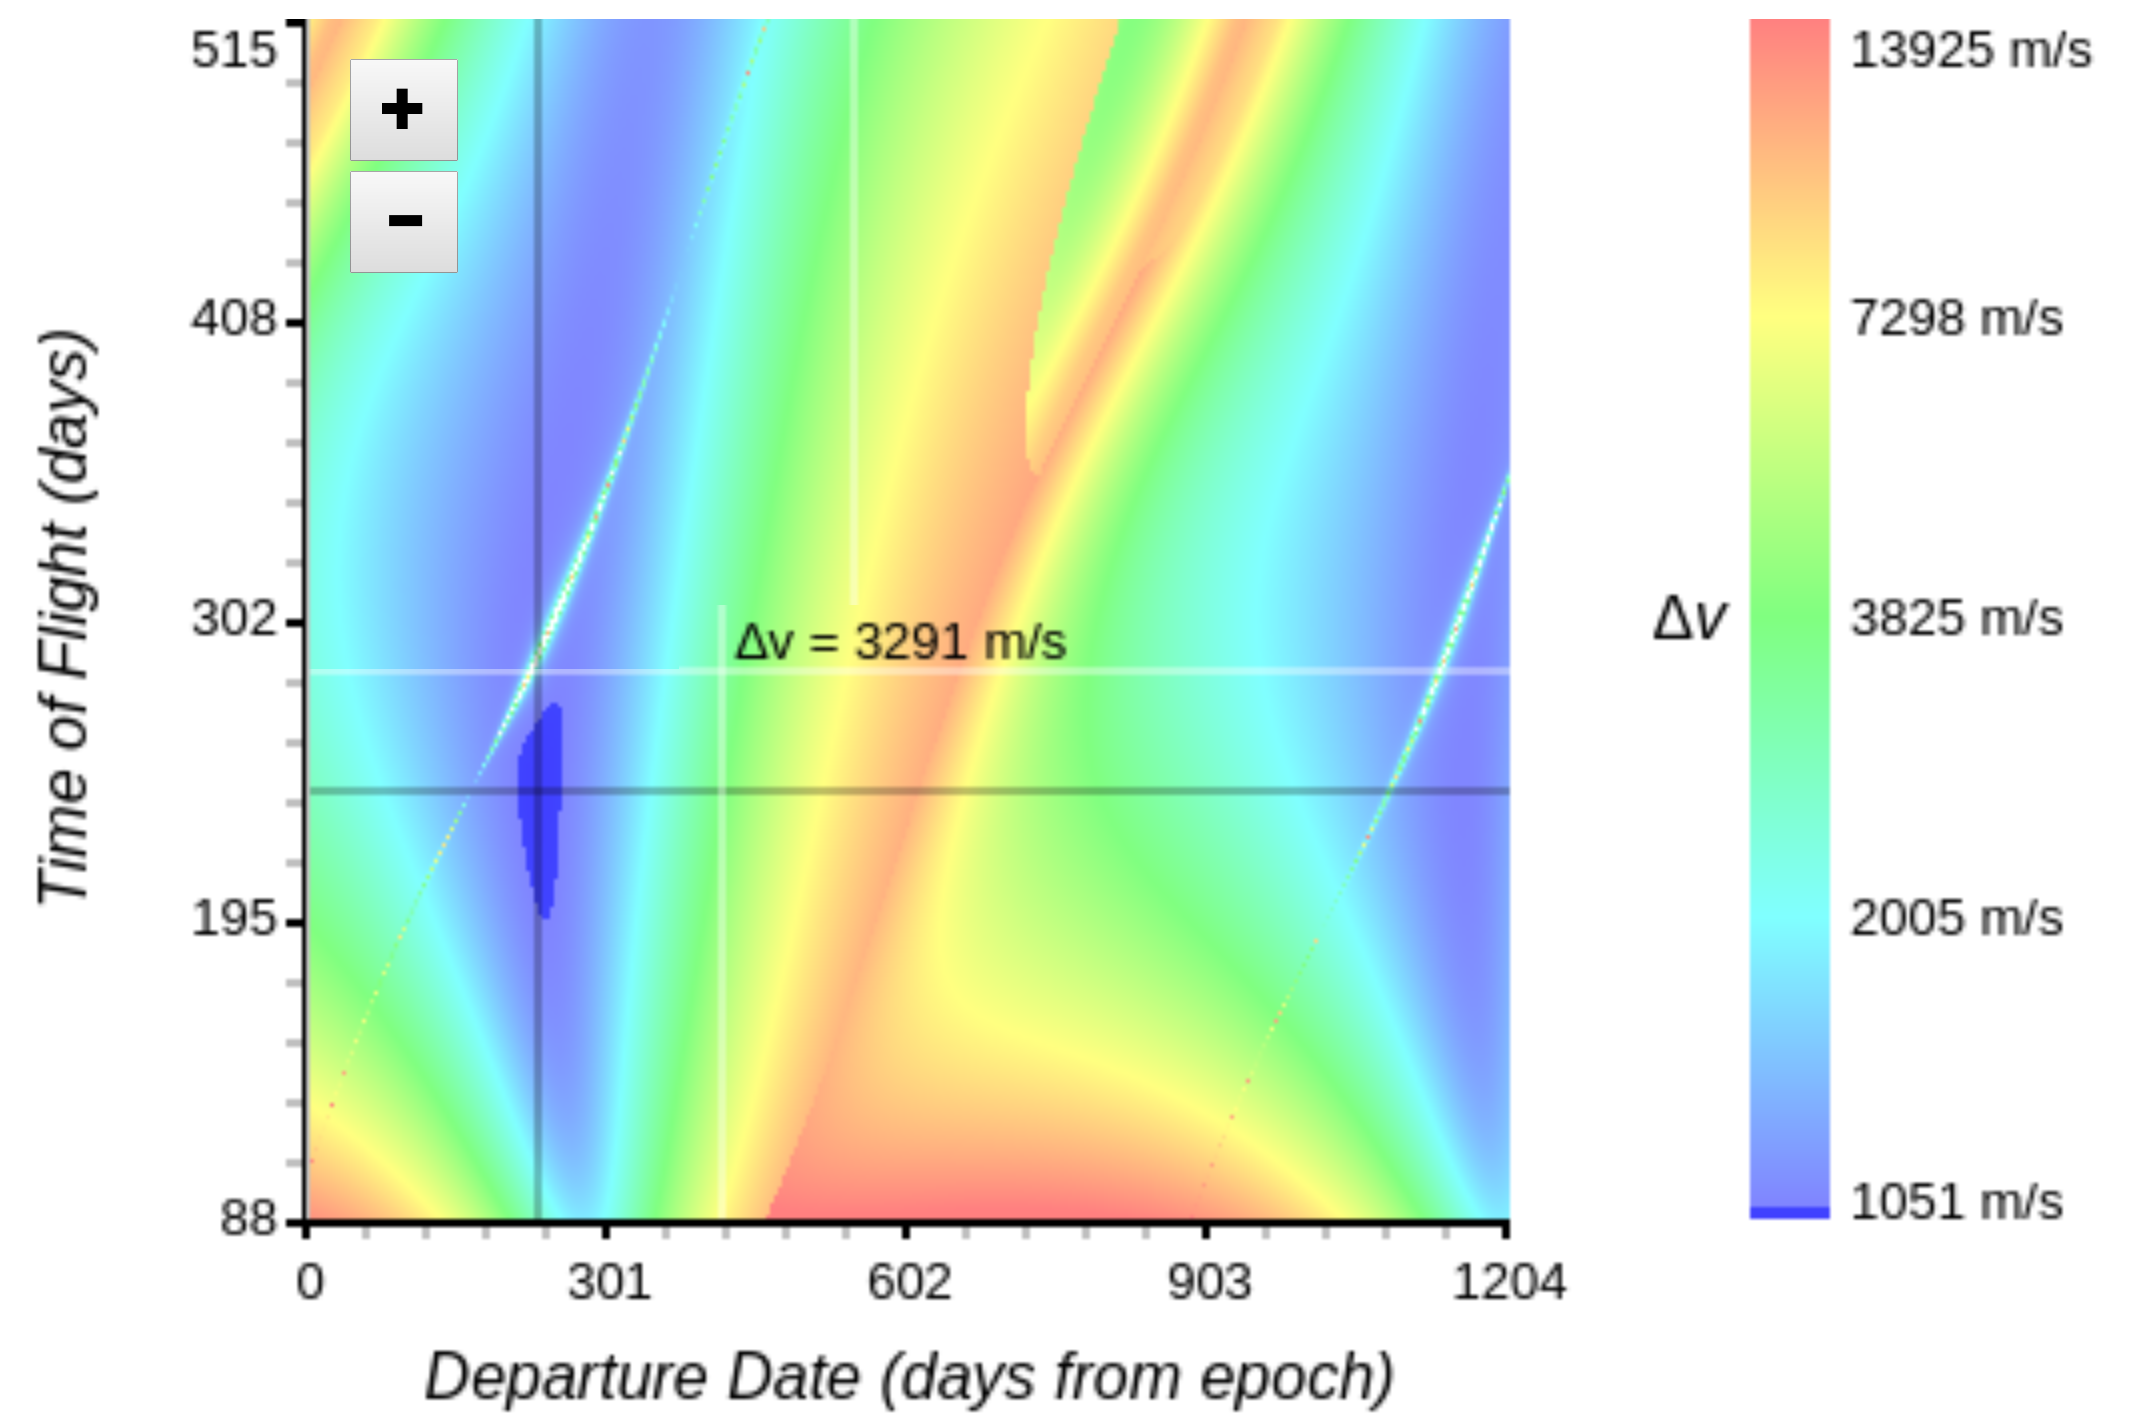
\includegraphics[scale=0.08]{images/hohmann_transfer_window}
        \end{center}
    \end{block}
\end{frame}
{
\usebackgroundtemplate{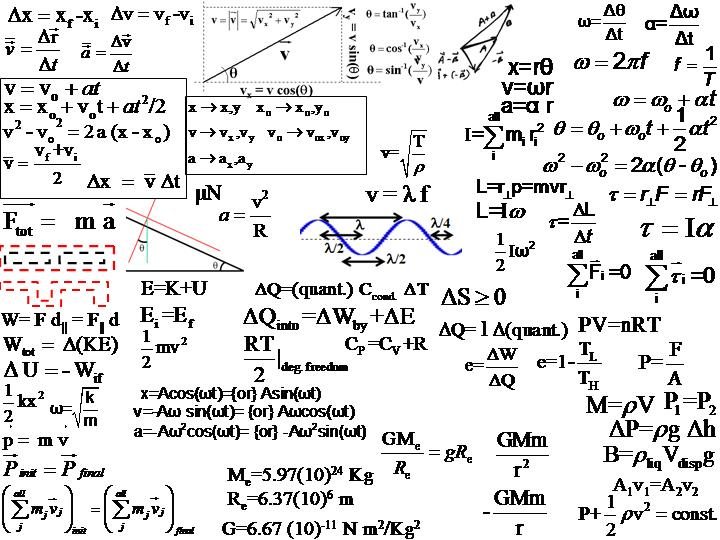
\includegraphics[width=\paperwidth]{images/oberth_troll}}%
\begin{frame}[t]{Oberth Effect}
\end{frame}
}
\begin{frame}[t]{JK, Oberth Effect}
    \begin{block}{}
        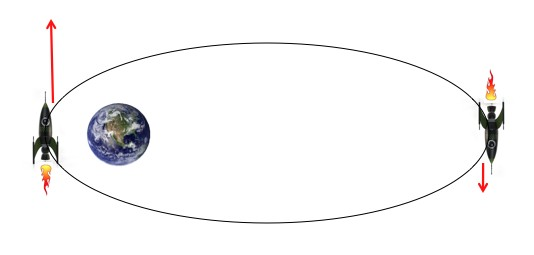
\includegraphics[width=\textwidth]{images/obert_effect}
    \end{block}
\end{frame}
\begin{frame}[t]{Oberth Effect explained}
    \begin{block}{}
        \begin{itemize}
            \item things that go fast have higher energy
            \item $KE = 0.5 * m * v^2$
        \end{itemize}
    \end{block}
    \begin{block}{}
        \begin{itemize}
            \item mass is a form of energy
            \item $E = MC^2$
        \end{itemize}
    \end{block}
    \begin{block}{}
        \begin{itemize}
            \item Newton's third law
            \item $F_a = -F_b$
        \end{itemize}
    \end{block}
    \begin{block}{}
        Dumping mass (fuel) while deep in the gravity well (going fast) gives more kinetic energy to the ship {\tiny
        This is an oversimplification}
    \end{block}
\end{frame}
\begin{frame}[t]{Escape}
    \begin{block}{}
        Now that we know how to make optimal use of the Oberth effect we can begin our escape burn and start our tranfer orbit
    \end{block}
    \begin{block}{}
        \begin{itemize}
            \item descelarate to drop periapsis deeper into the gravity well
            \item wait for periapsis (maximal use of Oberth effect)
            \item make transfer burn and coast to encounter
        \end{itemize}
    \end{block}
\end{frame}
